\documentclass[a4paper]{article}
\usepackage[english, russian]{babel}
\usepackage[utf8]{inputenc}
\usepackage{multicol}
\usepackage{float}
\usepackage{graphicx}
\usepackage[includeheadfoot]{geometry}
\usepackage{caption}
\usepackage{textcomp}
\usepackage{fancyhdr}
\usepackage{multirow}

\geometry{margin=1cm}
\setcounter{equation}{2}
\captionsetup[figure]{singlelinecheck=false, justification=RaggedRight, font=sl}



\begin{document}

\setcounter{page}{5}
\pagestyle{fancy}
\fancyhf{}
\fancyhead[R]{\large\thepage}
\fancyhead[C]{ГИПОТЕЗА ТАНИЯМЫ И ПОСЛЕДНЯЯ ТЕОРЕМА ФЕРМА}
\fancyfoot[L]{\scriptsize{2 Квант № 4}}
\renewcommand{\headrulewidth}{0pt}
\renewcommand{\arraystretch}{1.75}

\vspace*{-3.5\baselineskip}
\begin{multicols}{3}

\begin{figure}[H]
    \centering
    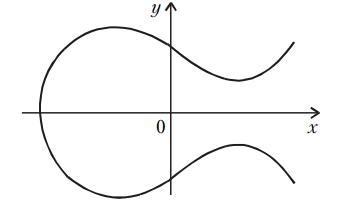
\includegraphics[width=\linewidth]{Рис.4.png}
    \caption*{Рис. 4}
\end{figure} 
\begin{figure}[H]
    \centering
    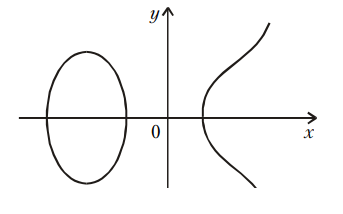
\includegraphics[width=\linewidth]{Рис.5.png}
    \caption*{Рис. 5}
\end{figure} 
\noindentДля кривой, заданной в каноничес-
кой форме (2), дискриминант \(\Delta\) определяется формулой \[\Delta=-(4a^3+27b^2).\]

Пусть $E$ - некоторая эллиптическая кривая, заданная уравнением \[y^2 = x^2 +ax+b,\] в котором $a$ и $b$ - целые числа. Для простого числа $p$ рассмотрим сравнение 
\begin{equation}
    y \equiv x^3 + \overline a x + \overline b \pmod{p}
\end{equation}
где \(\overline a\) и \(\overline b\) - остатки от деления целых
чисел $a$ и $b$ на $p$, и обозначим через \(n_p\) число решений этого сравнения. Числа  \(n_p\), очень полезны при исследовании вопроса о разрешимости уравнений вида (2) в целых числах: если какое-то \(n_p\) равно нулю, то уравнение (2) не имеет целочисленных решений. Однако вычислить числа  \(n_p\) удается лишь в редчайших случаях.
В то же время известно, что \(|p-n_p| \leq 2\sqrt{p}\) (теорема Хассе).

Рассмотрим те простые числа $p$, которые делят дискриминант \(\Delta\) эллиптической кривой (2). Можно доказать, что для таких р многочлен \(x^3 + \overline a x + \overline b\) можно записать одним из двух способов: \[x^3 + \overline a x + \overline b\equiv(x+\overline\alpha)^2(\overline\beta)\pmod{p}\] или \[x^3 + \overline a x + \overline b\equiv(x+\overline\gamma)^3\pmod{p},\] где \(\overline\alpha, \overline\beta, \overline\gamma\) - некоторые остатки от деления на p. Если для всех простых 

\columnbreak\noindent $p$, делящих дискриминант кривой, реализуется первая из двух указанныхных возможностей, то эллиптическая кривая называется \textit{полустабильной}.

Простые числа, делящие дискриминант, можно объединить в так называемый \textit{кондуктор} эллиптической кривой. Если $E$ - полустабильная кривая, то ее кондуктор $N$ задается формулой
\begin{equation}
    N = \prod_{p|\Delta}p^{\epsilon_p},
\end{equation}
где для всех простых чисел \(p \geq 5\), делящих \(\Delta\), показатель \(\epsilon_p\), равен 1. Показатели \(\epsilon_2\) и \(\epsilon_3\), вычисляются с помощью специального алгоритма.
\begin{center}
    \parbox{0.85\linewidth}{\centering\large\bfseries\sffamily{Модулярные формы\\и модулярные эллиптические кривые}}
\end{center}
Обозначим через H верхнюю комплексную полуплоскость. Пусть N - натуральное и k - целое числа. \textit{Модулярной параболической формой} веса k уровня N называется аналитическая функция f(z), заданная в верхней полуплоскости и удовлетворяющая соотношению
\begin{equation}
    f(\frac{az+b}{cz+d}) = (cz+d)^k f(z)
\end{equation}
для любых целых чисел $а, b, c, d$ таких, что \(ad - bc = 1\) и c делится на N. Кроме того, предполагается, что \[\lim\limits_{t \to +0}f(r+it)=0,\] где r - рациональное число, и что \[\lim\limits_{t \to \infty}f(it)=0.\]

Пространство модулярных параболических форм веса k уровня N обозначается через \(S_k(N)\). Можно показать, что оно имеет конечную размерность.

В дальнейшем нас будут особо интересовать модулярные параболические формы веса 2. Для малых N
размерность \(\dim S_2(N)\) простран-
ства \(S_2(N)\) представлена в таблице:
\begin{table}[H]
    \begin{tabular}{|c|c|c|c|c|c|c|} 
    \hline \textit{N} < 10 & 11 & 12 & 13 & 14 & 15 & 16 \\ \hline
    0 & 1 & 0 & 0 & 1 & 1 & 0 \\ \hline
     & 17 & 18 & 19 & 20 & 21 & 22 \\ \cline{2-7}
     & 1 & 0 & 1 & 1 & 1 & 2 \\ \hline
    \end{tabular} 
\end{table} 
\columnbreak\noindentВ частности, 
\begin{equation}
    \dim S_2(2) = 0.
\end{equation} 

Отметим, что эта нехитрая формула сыграет важную роль в доказательстве теоремы Ферма.

Из условия (5) следует, что $f(z + 1) = f(z)$ для каждой формы $f \in S_2(N)$. Стало быть, f является периодической функцией. Такую функцию можно представить в виде
\begin{equation}
    f(z)=\sum^\infty_{n=1}a_nq^n, q=e^{2\pi iz}.
\end{equation}

Назовем модулярную параболическую форму $f(z)\in S_2(N)$ собственной, если ее коэффициенты - целые числа, удовлетворяющие соотношениям \[a_1 =1;\]
\begin{center}
    \(a_{p^r}a_p = a_{p^{r+1}}pc_{p^{r-1}}\) для простого $p$,
    \begin{equation}
        \textup{не делящего число } N;
    \end{equation}
    \(a_{p^r} = (a_p)^r\) для простого $p$, \\делящего число $N$; 
    \[a_{mn}=a_ma_n, \textup{если} (m, n) = 1.\]    
\end{center}

Сформулируем теперь определение, играющее ключевую роль в доказательстве теоремы Ферма. Эллиптическая кривая с рациональными коэффициентами и кондуктором N называется \textit{модулярной}, если найдется такая собственная форма
\begin{equation}
    f(z)=\sum^\infty_{n=1}a_nq^n \in S_2(N),
\end{equation}
что \(a_p = p - n_p\) для почти все простых чисел p. Здесь $n_p$ - число решений сравнения (3).
\begin{center}
    \large\bfseries\sffamily{Гипотеза Таниямы}
\end{center}
Определение модулярной эллиптической кривой является настолько жестким, что на первый взгляд кажется невероятным существование хотя бы одной такой кривой. Трудно представить, что функция f(z), удовлетворяющая перечисленным выше весьма ограничительным условиям (5) и (8), разлагается в ряд (7), коэффициенты которого связаны с практически невычислимыми числами $n_p$. Однако эмпирический
материал, полученный в первой по-
\end{multicols}



\end{document}